\section{Methods}

Our methodology consisted of four main stages: dataset preparation, audio representation with the Audio Spectrogram Transformer (AST), multimodal alignment with CLIP, and dimensionality reduction with principal component analysis (PCA).

\subsection{Dataset}
We primarily used the Free Music Archive (FMA) dataset \cite{FMA}. FMA contains 106,574 tracks from 16,341 artists and 14,854 albums, spanning 161 genres. Training on such a diverse collection encouraged the model to generalize more effectively and produce more accurate embeddings for previously unheard audio.

\subsection{Audio Representation with AST}

Our training approach began with using a pre-trained version of the Audio Spectrogram Transformer (AST) developed by Gong et al \cite{AST}. This transformer first takes each .mp3 file from our dataset and converts it into a spectrogram. A spectrogram is a visual representation of audio, depicting the frequency and amplitude of the songs over time. It shows a greater level of detail than comparable visual representations such as waveforms, making it ideal for analyzing audio tracks in more depth \cite{spectrograms}.

\begin{figure}[ht]
  \centering
  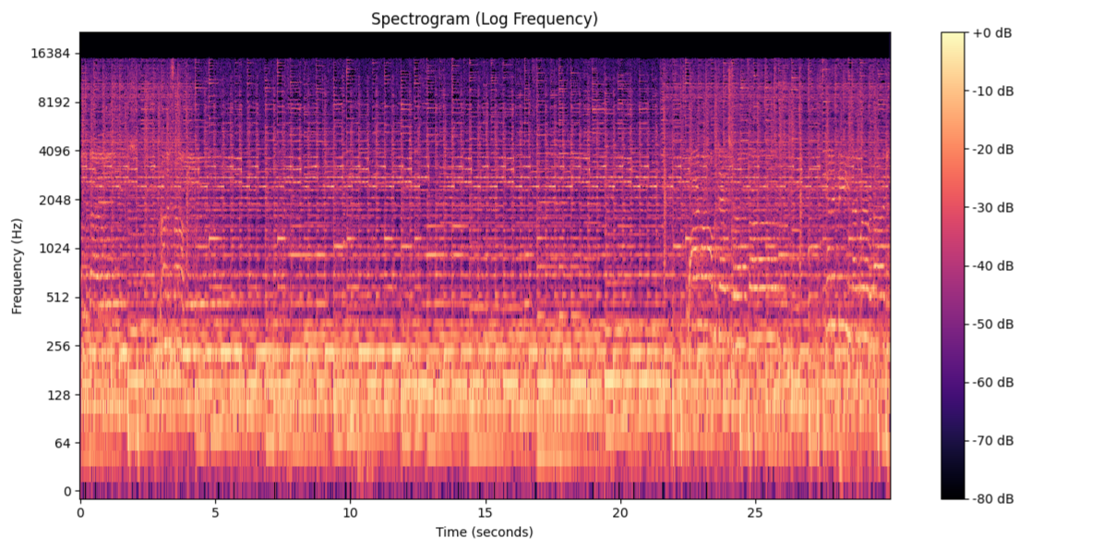
\includegraphics[width=0.8\linewidth]{figures/CallingForYouSpectro.png}

   \caption{An example spectrogram, similar to those generated by AST. It is a visual representation of one of our dataset tracks, "Calling For You" by The Twin Atlas.}
   \label{fig:onecol}
\end{figure}

Only using 30 second clips meant that every spectrogram shared the same scale and axes, resulting in more uniform training data. These smaller clip sizes were easier to process, but did not make full use of the AST’s ability to handle variable-length inputs. Overly-consistent training data may have also negatively affected the model’s ability to generalize, potentially factoring into reduced performance on testing data that did not fit the 30 second structure.

The AST divides each spectrogram into overlapping $16 \times 16$ image patches before linearly projecting them into one-dimensional patch embeddings. These patch embeddings are added with learnable positional embeddings and prepended with a classification token. The output embedding becomes the Transformer input, while the classification token is used with a linear layer for classification purposes \cite{AST}. Using this approach provided a valuable way to process audio in a visual format.

Notably, the AST was fine-tuned on AudioSet, a labeled dataset cultivated by Google that contains over two million audio clips. The items within AudioSet are sound events derived from YouTube, meaning that the model’s pre-trained weights required fine-tuning in order to better suit the music domain \cite{audioset}.

\subsection{Multimodal Alignment with CLIP}

The second major component of our multimodal approach was the Contrastive Language-Image Pretraining (CLIP) vision transformer. While  AST handled the audio-based visual component of our methodology, CLIP’s text processing allowed us to incorporate text input and semantic meaning. For every song that contained vocals, we generated a respective set of lyrics. These lyrics were passed as input to the CLIP model, which then produced a 512-dimension lyric vector. The 768-dimension audio vector produced by the AST was compressed to 512 dimensions in order to match the lyric vector’s dimensions \cite{CLIP}.

From there, the symmetric cross-entropy loss was computed and used to more closely align each audio vector with its respective lyric vector. We followed a similar approach to Radford et al., using a temperature to allow the model to be flexible with the way it handles distances and forms clusters \cite{CLIP}. Once loss is computed, backpropagation passes the value back through the network to determine the gradient and reduce the loss in the next iteration. Following standard protocol for Transformer models, AdamW was used to update the model weights using a combination of momentum and scaling with added weight decay \cite{adamW}.

\subsection{Principal Component Analysis}

The resulting 512-dimensional output was centered and condensed to prime the embeddings for principal component analysis. The axes, PC1, PC2, and PC3, are calculated in order to show the greatest variance between data points. Once the axes are determined, all resulting vectors are projected onto the PCA space. As a linear approach, PCA gave us a more interpretable output while reducing the risk of imaginary clusters sometimes seen with UMAP or t-SNE \cite{PCA} \cite{dimensionality}.

\begin{figure}[ht]
  \centering
  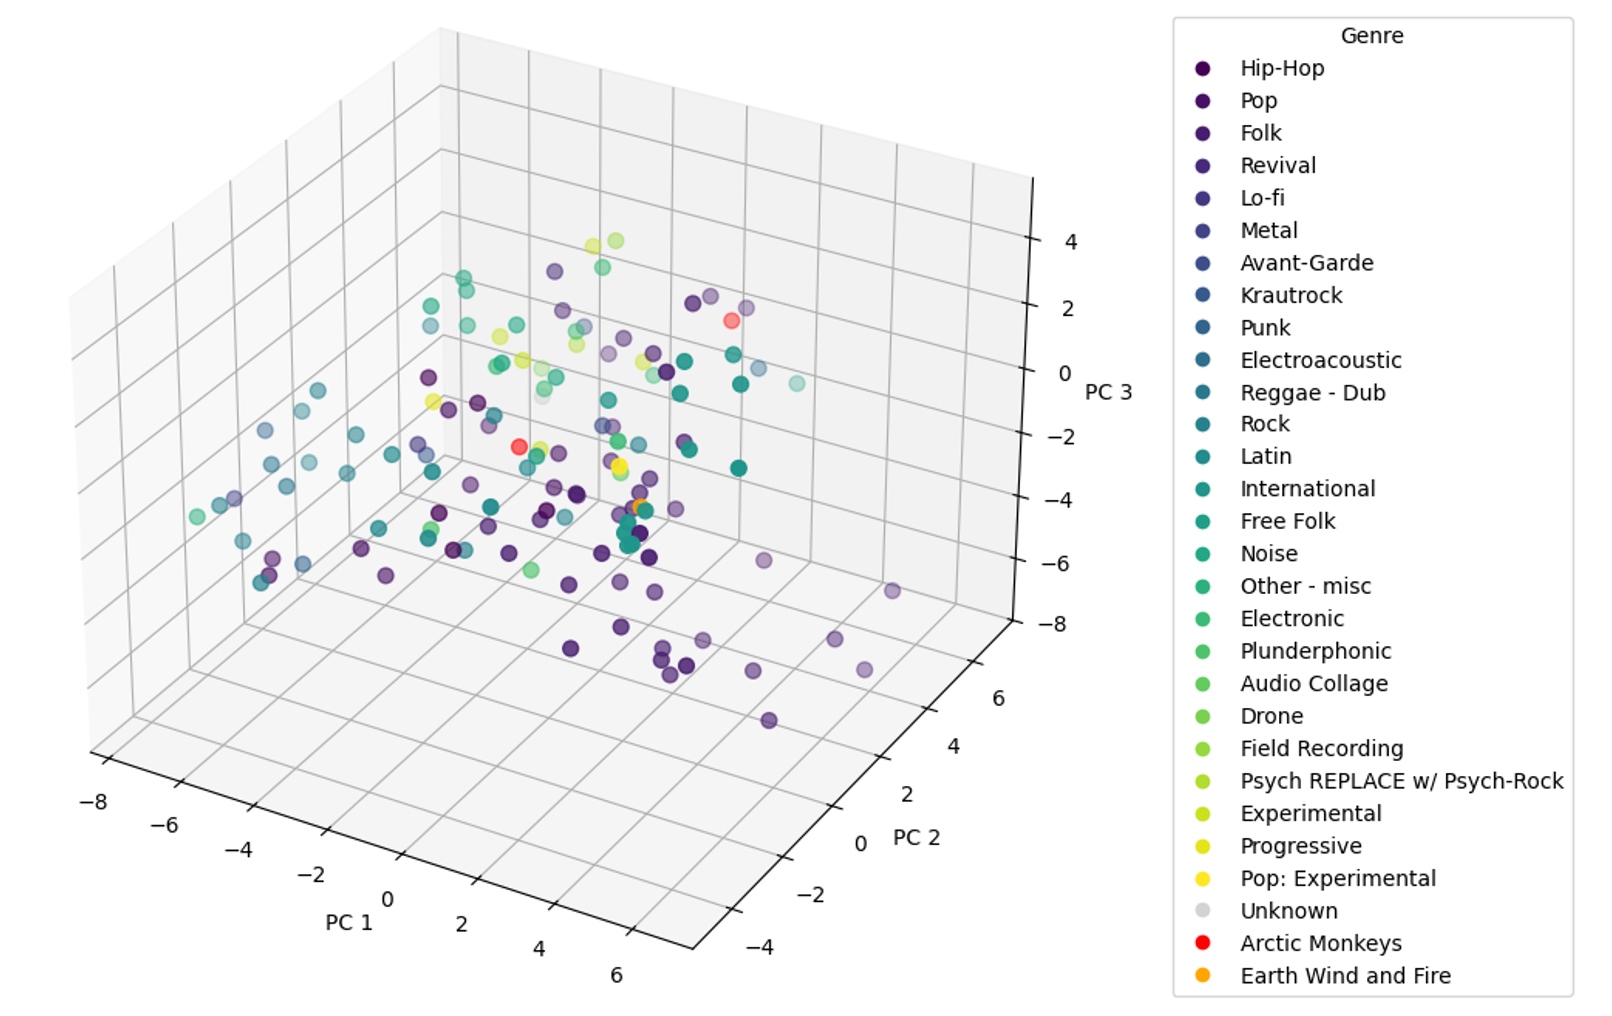
\includegraphics[width=0.8\linewidth]{figures/PCABefore.png}

   \caption{The PCA projection of a small subset of data with genres distinguished by color.}
   \label{fig:onecol}
\end{figure}
